% MASTER KINEMATIC CHAIN. Seven joints in an alternating roll/bend pattern,
% with the measured link lengths. Drawn straight (all joints at zero) so the
% lengths can be read off directly.
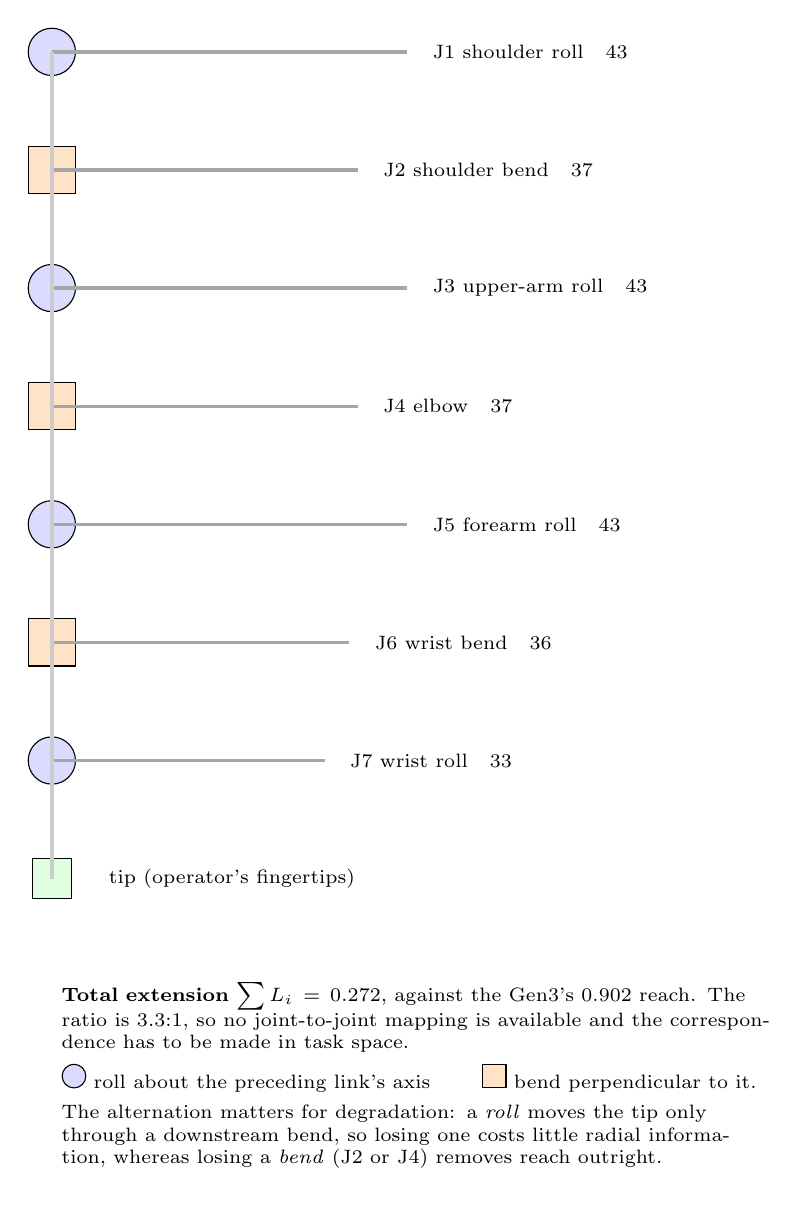
\begin{tikzpicture}[x=1mm, y=1mm, font=\scriptsize]

% The joint style is carried as a loop variable by NAME. Passing the style
% body directly fails: \foreach strips the braces and TikZ then reads the
% comma inside "circle, fill=blue!14" as an option separator, so "circle" is
% parsed as a colour.
\tikzset{
  jroll/.style = {draw, circle, fill=blue!14, minimum size=6mm, inner sep=0pt},
  jbend/.style = {draw, fill=orange!22, minimum size=6mm, inner sep=0pt},
}
\foreach \i/\len/\sty/\name in {
  1/43/jroll/{J1 shoulder roll},
  2/37/jbend/{J2 shoulder bend},
  3/43/jroll/{J3 upper-arm roll},
  4/37/jbend/{J4 elbow},
  5/43/jroll/{J5 forearm roll},
  6/36/jbend/{J6 wrist bend},
  7/33/jroll/{J7 wrist roll}}
{
  \pgfmathsetmacro{\y}{-\i*15}
  \pgfmathsetmacro{\w}{\len*1.05}
  \node[\sty] (j\i) at (0, \y) {};
  \draw[very thick, gray!70] (0,\y) -- (\w, \y);
  \node[anchor=west, font=\scriptsize] at (\w+2, \y)
     {\name \quad \SI{\len}{\milli\metre}};
}

\node[draw, fill=green!12, minimum size=5mm, inner sep=1pt] (tip) at (0, -120) {};
\node[anchor=west] at (6, -120) {tip (operator's fingertips)};

\draw[very thick, gray!40] (0,-15) -- (0,-120);

\node[anchor=north west, text width=90mm, align=left] at (0, -132)
  {\textbf{Total extension} $\sum L_i = \SI{0.272}{\metre}$, against the Gen3's
   \SI{0.902}{\metre} reach. The ratio is 3.3:1, so no joint-to-joint mapping
   is available and the correspondence has to be made in task space.\\[3pt]
   \tikz\node[draw, circle, fill=blue!14, minimum size=3mm, inner sep=0pt]{};\ %
   roll about the preceding link's axis \qquad
   \tikz\node[draw, fill=orange!22, minimum size=3mm, inner sep=0pt]{};\ %
   bend perpendicular to it.\\[3pt]
   The alternation matters for degradation: a \emph{roll} moves the tip only
   through a downstream bend, so losing one costs little radial information,
   whereas losing a \emph{bend} (J2 or J4) removes reach outright.};
\end{tikzpicture}
